\apendice{Plan de Proyecto Software}

\section{Introducción}

El objetivo de este proyecto es realizar un simulador de como genera el árbol de decisión el algoritmo C4.5 o también conocido como J48 con Weka.

El algoritmo C4.5 se utiliza para generar el árbol de decisión de un conjunto de datos, este conjunto de datos tiene diferentes variables, pero se distinguen en dos grupos, el primer grupo son las variables decisión, que son las variables que nosotros escogemos para elegir el camino y la variable objetivo, que es la variable que nosotros escogemos como variable que nos indica que resultado obtenemos de haber elegido ese camino.

\section{Planificación temporal}

\subsection{\textit{Sprint} 1 (16/03/2026 - 07/04/2026): Arreglos y Comienzo del desarrollo}

\paragraph{Objetivos}
Los objetivos principales de este $\textit{sprint}$ fueron arreglar tanto la configuración de la herramienta de $Zube$ como la configuración del repositorio con la sección de $Actions$, para que el despliegue de la web sea haga de forma automática y sin tener que realizar ningún tipo de ajuste adicional.

\begin{figure}[htbp]
     \centering
     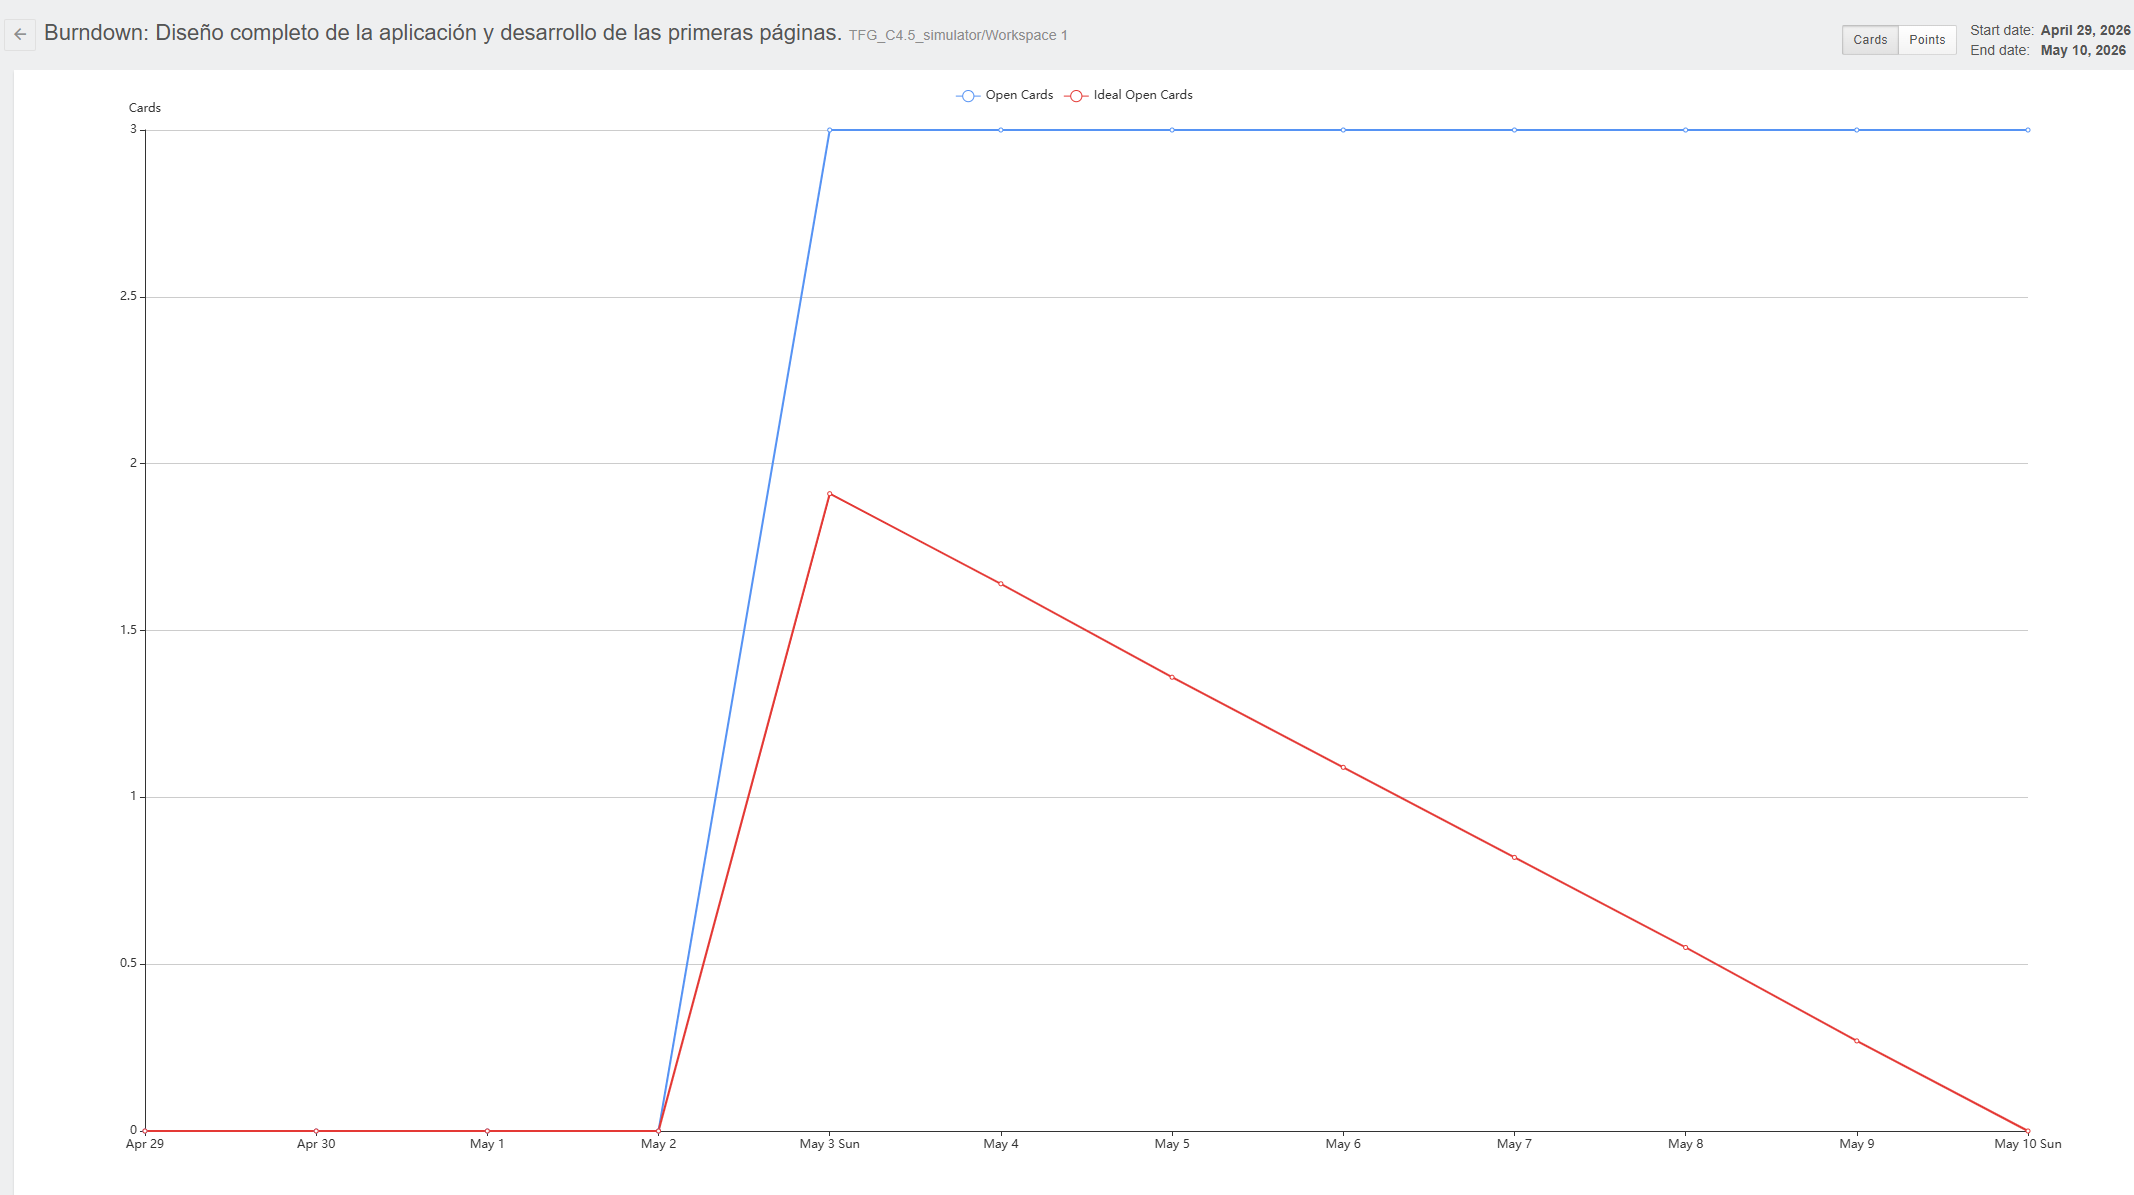
\includegraphics[width=0.75\textwidth]{img/burndown_zube_1.png}
     \caption{\textit{Burndown del \textit{sprint} 1}}
     \label{Fig_A.1}
 \end{figure}


\paragraph{Resultado}
Arreglado todo lo referente a las Actions y definición de el siguiente \textit{sprint}, además, de diferentes sugerencias de mejora por parte de los tutores.

\subsection{\textit{Sprint} 2 (29/04/2026 - 10/05/2026): Diseño de la aplicación y desarrollo de las primeras secciones}

\paragraph{Objetivos}
Los objetivos principales de este \textit{sprint} fueron diseñar la interfaz de la aplicación en la herramienta de $Figma$ así como diseñar el formato de la aplicación para la simulación del algoritmo, ademas de empezar con el desarrollo de las secciones para poder aplicar cambios o mejoras necesarias para futuros \textit{sprint}

\begin{figure}[htbp]
     \centering
     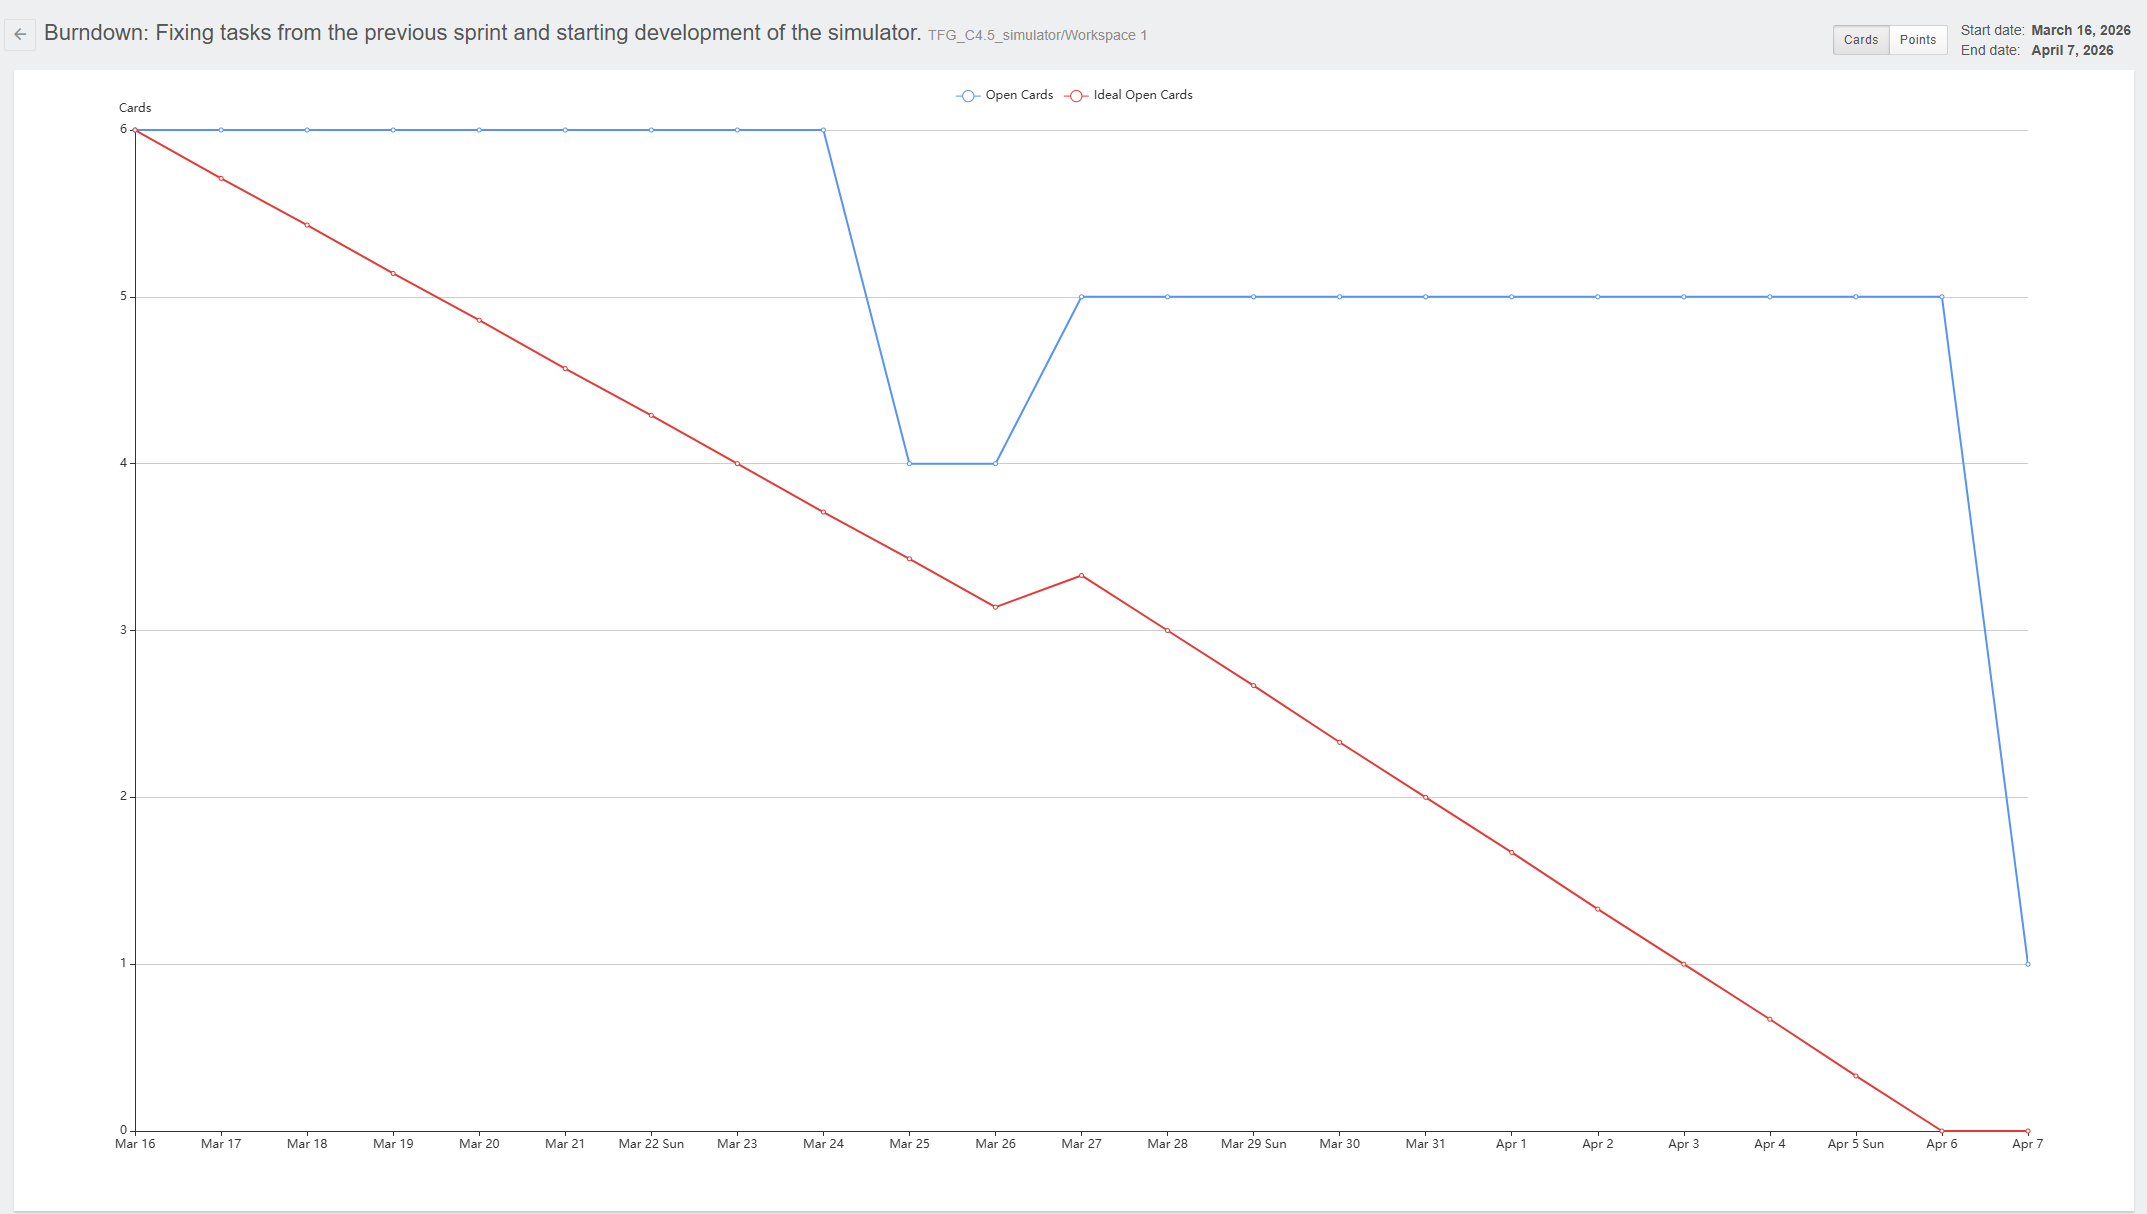
\includegraphics[width=0.75\textwidth]{img/burndown_zube_2.png}
     \caption{\textit{Burndown del \textit{sprint} 2}}
     \label{Fig_A.3}
 \end{figure}

\paragraph{Resultado}
Creación del diseño de la aplicación, cambios generales en la parte de la sección de elección de nodos y cambios en el diseño de la web para unificar el formato de toda la web

\subsection{\textit{Sprint} 3 (19/05/2026 - 26/05/2026): Arreglos del anterior \textit{sprint} y continuar con el desarrollo}

\paragraph{Objetivos}
Los objetivos de este \textit{Sprint} fueron modificar todo lo referente al segundo \textit{sprint} e implementar las mejoras en la web, ademas de avanzar con al documentación del proyecto.

\begin{figure}[htbp]
     \centering
     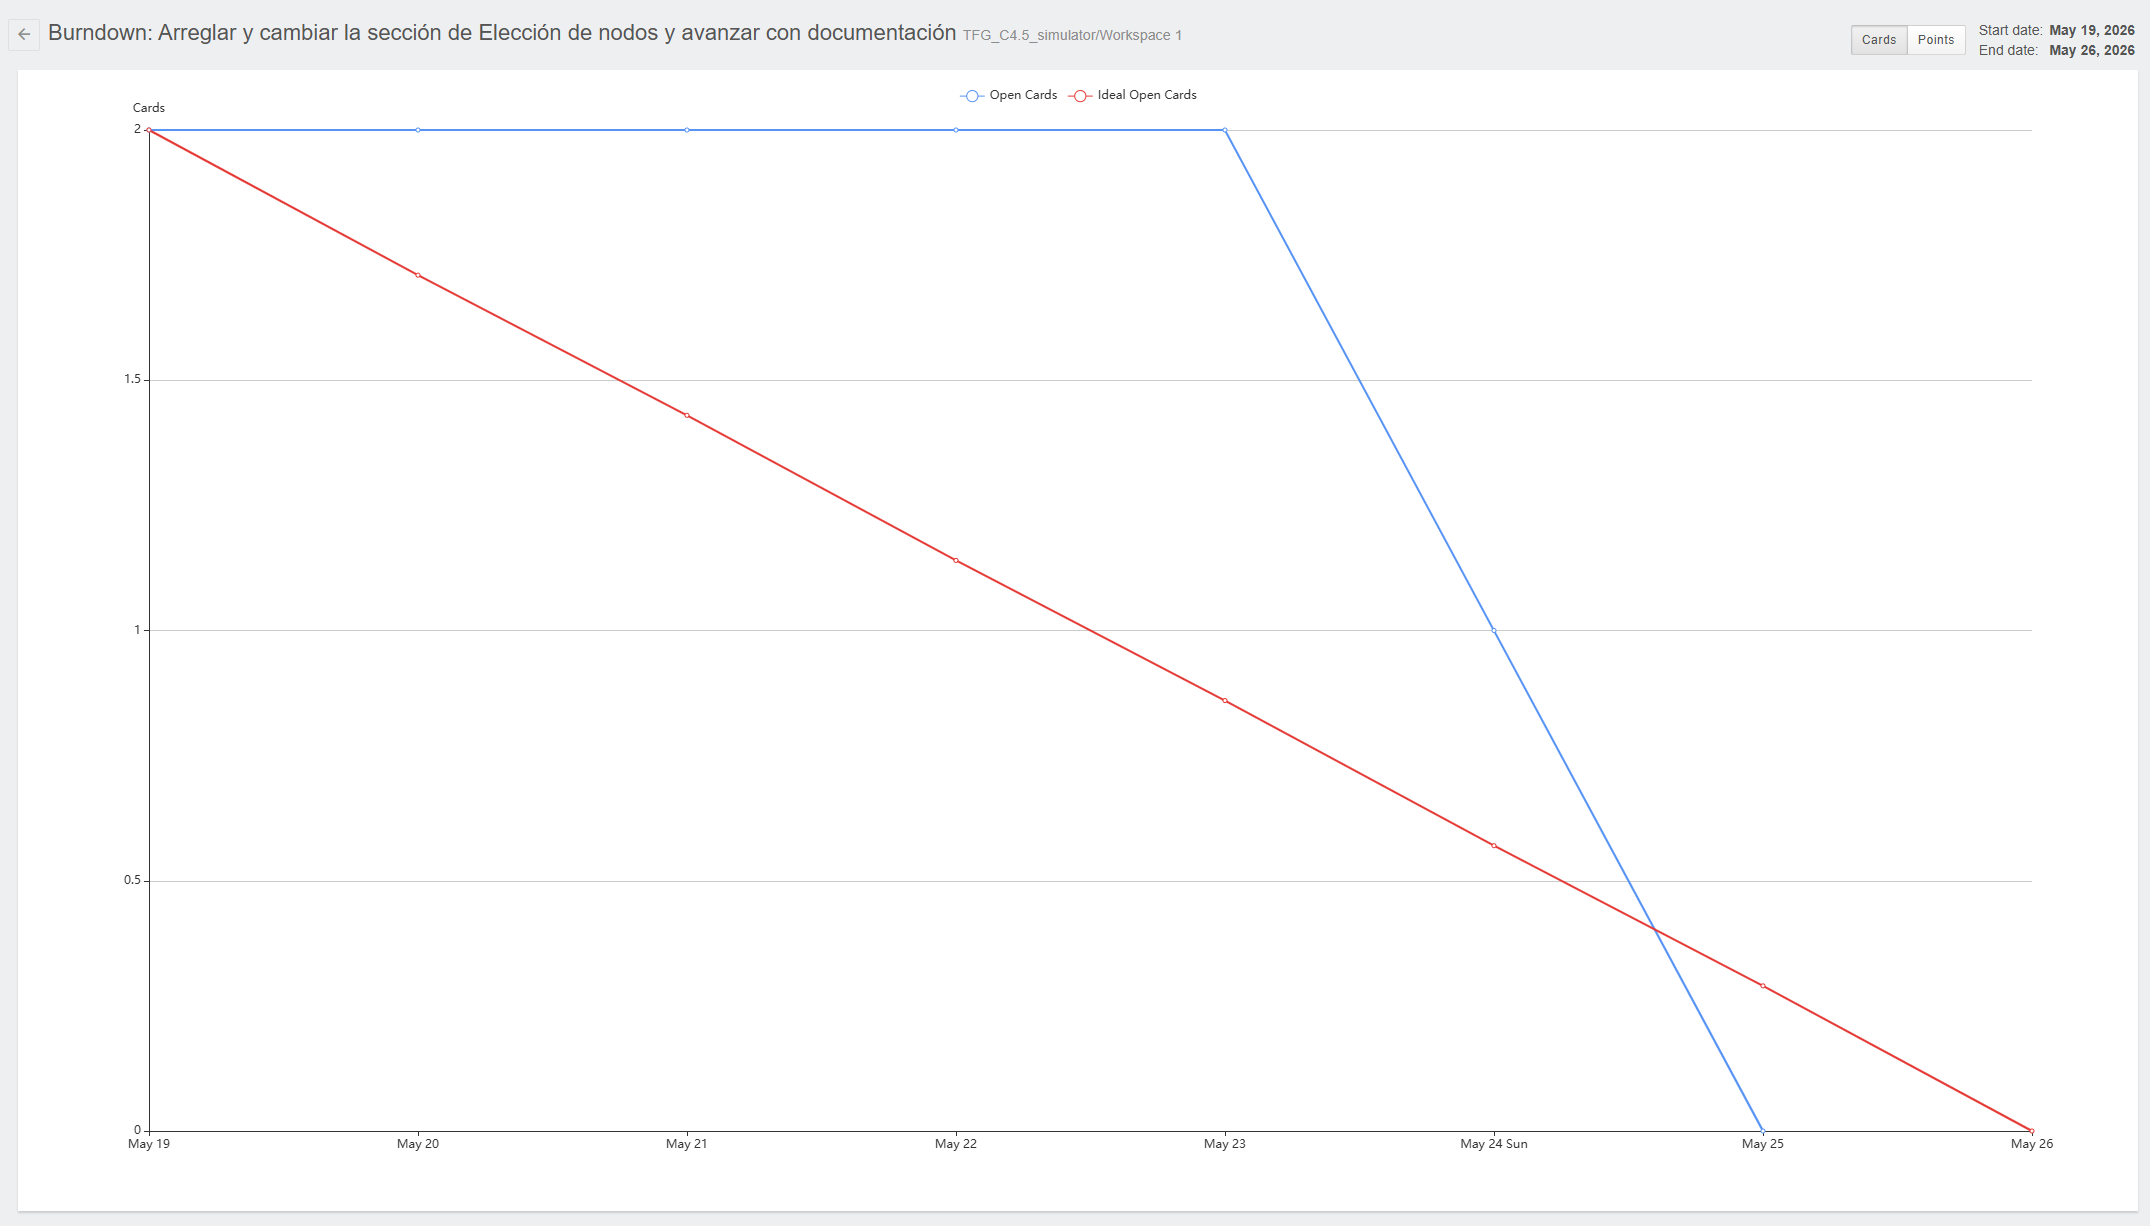
\includegraphics[width=0.75\textwidth]{img/burndown_zube_3.png}
     \caption{\textit{Burndown del \textit{sprint} 3}}
     \label{Fig_A.3}
 \end{figure}
 
\paragraph{Resultado}
Se realizaron los cambios pertinentes en la sección de elección de nodo y se continuo de manera breve con la documentación

\subsection{\textit{Sprint} 4 (30/05/2026 - 8/06/2026): Ampliar memoria y realizar cambios en la sección de elección de nodos}

\paragraph{Objetivos}
Los objetivos de este \textit{sprint} se fijaron principalmente en la mejora de la sección de elección de nodos, principalmente en la mejora visual y la organización de los elementos de la página para la experiencia de usuario.

Una de las principales tareas fue la de crear una imagen con \textit{SVG} para visualizar el nodo que el algoritmo elige en la correspondiente sección, fue una tarea un poco complicada ya que tenia que cuadrar perfectamente y no ser demasiado grande para que el usuario pueda visualizar tanto el nodo elegido como los datos que llevan a elegir el nodo.

También uno de los arreglos más útiles de este \textit{sprint} fue el de añadir diferentes leyendas a las tablas y a las secciones para que el usuario pudiera tener referencias de lo que se está visualizando en pantalla y no perderse en la explicación de la sección

Con respecto al avance de la documentación, se pretendía avanzar en el apartado de Técnicas y herramientas para determinar el formato que debería de seguir en este apartado de la documentación.

\begin{figure}[htbp]
     \centering
     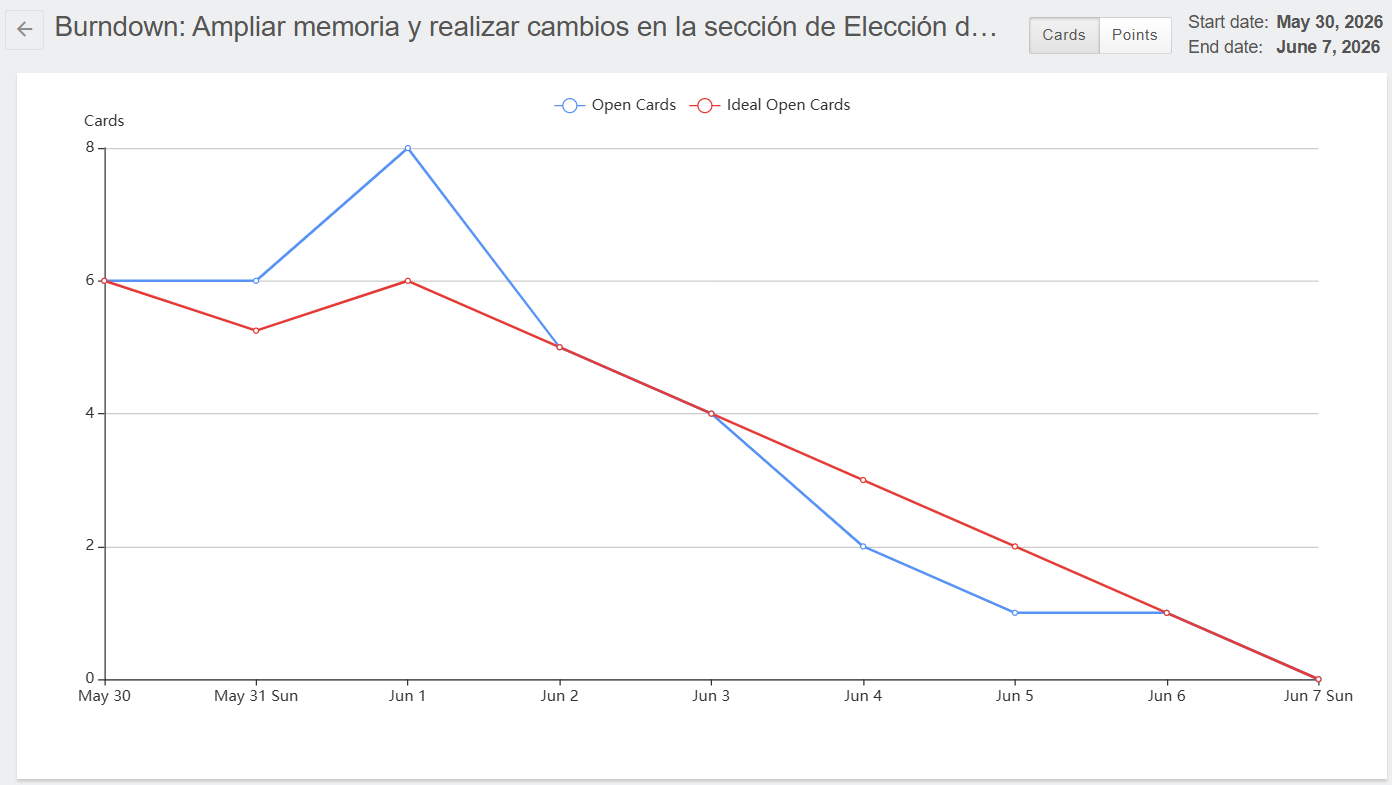
\includegraphics[width=0.75\textwidth]{img/burndown_zube_4.png}
     \caption{\textit{Burndown del \textit{sprint} 4}}
     \label{Fig_A.4}
 \end{figure}
 
\paragraph{Resultado}
Se realizaron los cambios de la web que indicaba el \textit{sprint}, dando por finalizado la sección de elección de nodo. Además, se realizaron correcciones en la parte de la documentación.

\subsection{\textit{Sprint} 5 (13/06/2026 - 24/06/2026): Desarrollo de la sección árbol de decisión C4.5 y continuación de la memoria}

\paragraph{Objetivos}
Los objetivos de este \textit{sprint} principalmente se basaron en el desarrollo de la sección para la simulación del árbol C4.5, dando una primera aproximación de como debería de quedar la sección para la finalización del proyecto.

En este sprint, el mayor reto fue cuadrar todas las secciones necesarias para la comprensión de la simulación del árbol paso a paso, se dio una aproximación dejando 3 secciones diferenciadas para la visualización del árbol, el \textit{dataset} que se estaba analizando y el conjunto de cálculos necesarios para entender el árbol.

Otro de los puntos de este \textit{sprint} fue aplicar todo lo dicho en el anterior \textit{sprint} con respecto a la sección de Técnicas y herramientas de la documentación, dejando este apartado pendiente para su revisión en el proximo sprint.

\begin{figure}[htbp]
     \centering
     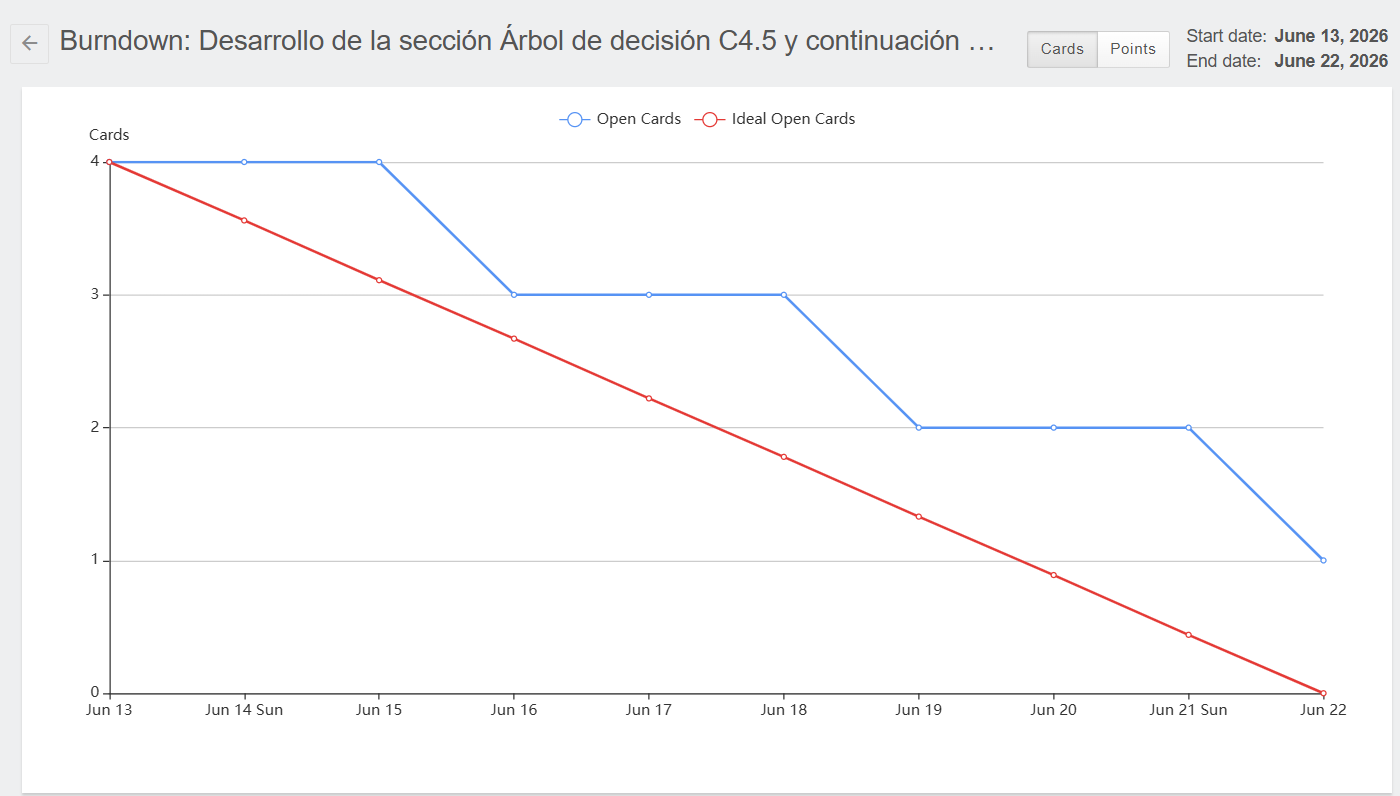
\includegraphics[width=0.75\textwidth]{img/burndown_zube_5.png}
     \caption{\textit{Burndown del \textit{sprint} 5}}
     \label{Fig_A.5}
 \end{figure}
 
\paragraph{Resultado}
Se dio una primera aproximación de lo que podría ser la sección de la generación del árbol y se dejaron pendientes de revisión los arreglos relacionados con la documentación. Además, de que se llegó a la conclusión de que se deberían de diferenciar la generación del árbol con la poda del mismo, ya que, en la misma página, no cabría la posibilidad de concentrar tanta información para que el usuario pueda llegar a entenderla.

\subsection{\textit{Sprint} 6 (24/06/2026 - 01/07/2026): Finalización del desarrollo y documentación}

\paragraph{Objetivos}
Los objetivos de este \textit{sprint} fueron aplicar diferentes mejoras visuales para la visualización de las secciones del árbol, el \textit{dataset} y los cálculos, además de finalizar el desarrollo del apartado de la poda.

El principal problema de este \textit{sprint} fue dejar una manera clara y visual la parte del árbol, para ello, se realizaron diferentes arreglos como la implementación de paneles retráctiles para las diferentes secciones y el uso del \textit{zoom} para la visualización de árboles grandes.

Se terminó la página de la poda siguiendo el mismo esquema visual que el usado en el apartado de la simulación del árbol, siendo la visualización de los cálculos necesarios para comprender este paso la parte más complicada del esta sección.

\begin{figure}[htbp]
     \centering
     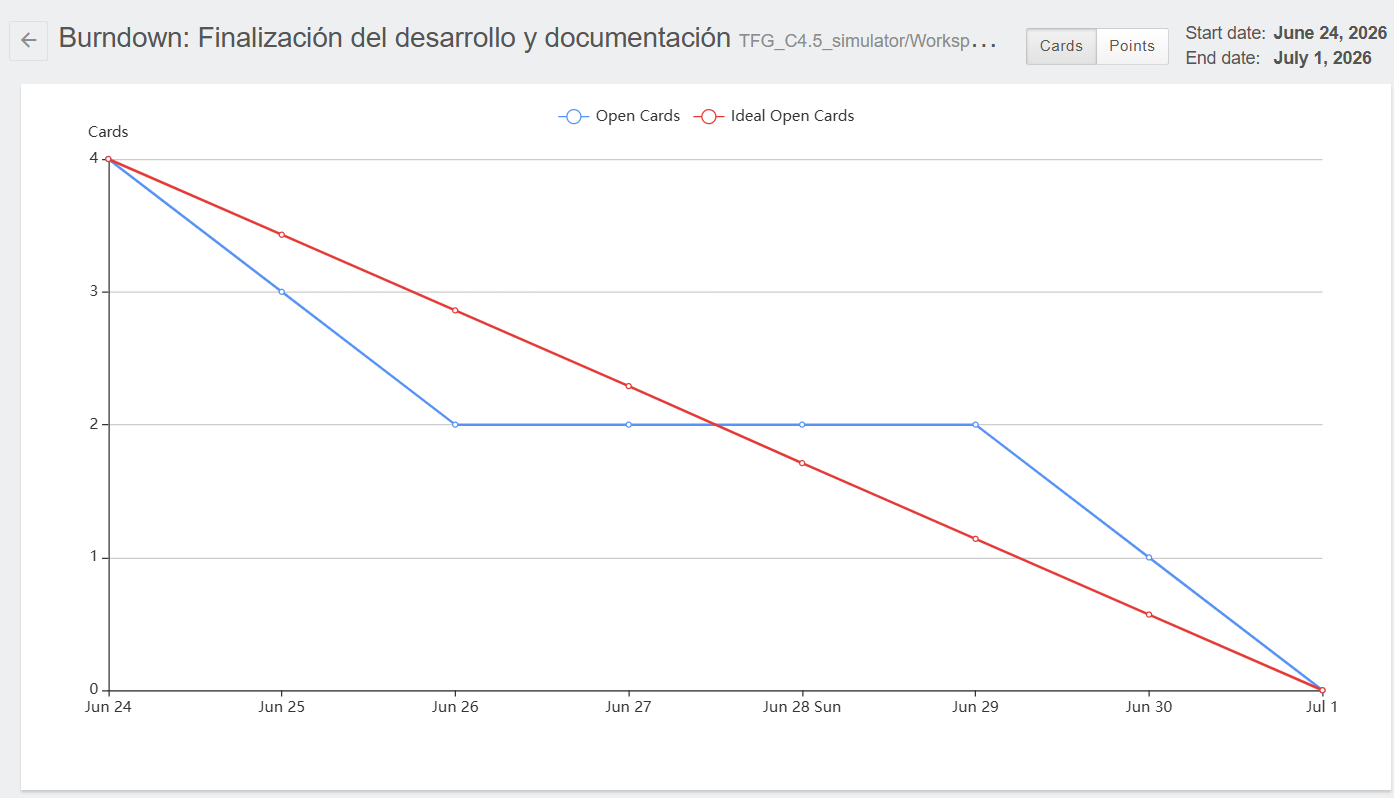
\includegraphics[width=0.75\textwidth]{img/burndown_zube_6.png}
     \caption{\textit{Burndown del \textit{sprint} 6}}
     \label{Fig_A.6}
 \end{figure}
 
\paragraph{Resultado}

Se realizaron todos los cambios pertinentes de la página web y se definió diferentes mejoras de bugs encontrados en la revisión de este \textit{sprint} además de dejar finalizada la parte de la web, se definió la realización de la documentación para finalizar el proyecto.


\section{Estudio de viabilidad}

\subsection{Viabilidad económica}

Este proyecto ha sido desarrollado por un programador a tiempo completo durante un período aproximado de 5 meses. Para estimar los costes de personal, se ha tomado como referencia el Salario Mínimo Interprofesional (SMI) vigente en España para el año 2026, fijado en 1.221 € mensuales en 14 pagas \cite{smi2026}. Tomando este salario como referencia, el coste salarial estimado sería:

\[
5m \times 1221\text{€}/m = 6105\text{€}
\]

Dado que esta cantidad representa únicamente el salario bruto, es necesario añadir las cotizaciones a la Seguridad Social. Considerando una carga total aproximada del 36,85\%, el coste total de personal asciende a:

\[
6105\text{€} + 6105\text{€} \times 0,3685 = 8354,69\text{€}
\]

\subsubsection{Costes de software y hardware}
\label{software_hardware_costs}

El coste de software de este proyecto es de 0€, ya que únicamente se han utilizado herramientas y aplicaciones de software libre o gratuitas.

En cuanto al hardware, se ha empleado un ordenador portátil con un valor de adquisición de 1.000€. Al haber sido utilizado durante todo el desarrollo del proyecto, cuya duración ha sido de 5 meses, se considera el siguiente coste asociado:

\[
1000\text{€}
\]

\subsubsection{Coste total}

Sumando los costes de personal y hardware, el coste total estimado del proyecto es:

\[
8354,69\text{€} + 1000\text{€} = 9354,69\text{€}
\]

\subsection{Viabilidad legal}

\subsubsection{Licencias de software utilizado}

Durante el desarrollo de la aplicación web, se han utilizado herramientas de software gratuitas que permiten su utilización con fines académicos y de desarrollo.

Las principales herramientas que se han utilizado son:

\begin{itemize}
    \item Visual Studio Code.
    \item Figma \footnote{Figma:\url{https://www.figma.com/design/pQNrLJYf1DwqGpvJNRfgGa/El-equipo-de-mga1010-team-library?node-id=3423-1202&t=21gWT3jmex66RqZt-0}}
    \item GitHub
    \item Zube \footnote{Zube:\url{https://zube.io/uni-2/tfg_c45_simulator/w/workspace-1/kanban}}
    \item ChatGPT
\end{itemize}

Todas estas herramientas disponen de planes gratuitos que permiten desarrollar proyectos personales y académicos por lo que en la utilización de este Trabajo Fin de Grado no supone ninguna infracción de licencias ni costes asociados a ellas.

\subsubsection{Propiedad Intelectual}

Todo el código fuente, documentación y recursos desarrollados específicamente para este proyecto son propiedad intelectual del su autor.

Todos los recursos utilizados para este proyecto de terceros, mantienen sus respectivas licencias de uso, respetándose en todo momento las condiciones establecidas por sus propietarios.

\subsubsection{Protección de datos}

La aplicación no almacena ni procesa datos personales de ningún tipo, por lo que no se incumple ninguno de los siguientes reglamentos:

\begin{itemize}
    \item Reglamento General de Protección de Datos (RGPD) \cite{rgpd2016}.
    \item Agencia Española de Protección de Datos \cite{lopdgdd2018}.
\end{itemize}

\subsubsection{Seguridad de la información}

El proyecto ha sido desarrollado siguiendo buenas prácticas de desarrollo seguro, incluyendo:

\begin{itemize}
    \item Controles de versiones mediante GitHub.
    \item Gestión de accesos mediante autenticación en plataformas utilizadas.
    \item Almacenamiento seguro del código fuente en repositorios privados o controlados.
\end{itemize}


